\documentclass[12pt]{article}

\usepackage[utf8]{inputenc}
\usepackage{latexsym,amsfonts,amssymb,amsthm,amsmath,graphicx,mathtools,subfig,hyperref}
\usepackage[parfill]{parskip}
\usepackage[export]{adjustbox}
\usepackage[justification=centering]{caption}
\usepackage{nameref}

\hypersetup{
    colorlinks=true,
    linkcolor=blue,
    filecolor=magenta,      
    urlcolor=cyan,
}

\DeclareMathAlphabet{\mymathbb}{U}{BOONDOX-ds}{m}{n}

\setlength{\parindent}{0in}
\setlength{\oddsidemargin}{0in}
\setlength{\textwidth}{17cm}
\setlength{\textheight}{22cm}
\setlength{\topmargin}{0cm}
\setlength{\headheight}{0pt}
\setlength{\footskip}{30pt}

\newcommand{\figw}{7cm}
\newcommand{\nnperfw}{7cm}

\title{EE-556 Homework 2}
\author{Edoardo Debenedetti}

\begin{document}

\maketitle

\section{Minimax problems and GANs}

\subsection{Minimax problem}

Consider the function $f : \mathbb{R}^2 \rightarrow \mathbb{R}$, where $f(x, y) = xy$.

\subsubsection{First order stationary points of \texorpdfstring{$f$}{Lg}}

In order to find the first order stationary points, we need to find the gradient and see with which $x$ and $y$ it is equal to $(0, 0)$. The gradient of $f$ is:
\begin{equation} \label{eq:f_gradient}
    \nabla f(x, y) = \left [ \frac{\partial}{\partial x} xy, \frac{\partial}{\partial y} xy \right] = [y, x]
\end{equation}
Clearly $\nabla f = (0, 0) \iff (x, y) = (0, 0)$. In order to classify this stationary point, we need to find the hessian of $f(0, 0)$:
\begin{equation} \label{eq:hessian_f}
    \nabla^2f(x, y) = \nabla \cdot \nabla f(x, y) =
        \left [ \frac{\partial}{\partial x}, \frac{\partial}{\partial y} \right]
        \cdot \begin{bmatrix} y \\ x \end{bmatrix} = 
        \begin{bmatrix} 0 & 1 \\ 1 & 0 \end{bmatrix} \ \forall x,  y \in \mathbb{R}
\end{equation}
The eigenvalues of $\nabla^2f(x, y)$ are $\lambda_{1} = -1$ and $\lambda_{2} = 1$, one is positive and one is negative, hence the matrix is not (semi-)positive nor (semi-)negative definite. However, we can do the second derivative test to say something more:
\begin{equation} \label{eq:f_hessian_det}
    Df(x, y) = \frac{\partial^2 f}{\partial^2 x} \frac{\partial^2 f}{\partial^2 y} - 
        \frac{\partial^2 f}{\partial x \partial y} \frac{\partial^2 f}{\partial y \partial x} = 0 \cdot 0 - 4 \cdot 1 = -4
\end{equation}
Since $Df(0, 0) < 0$, $(0, 0)$ is a saddle point.

\subsubsection{Solution of minimax problem \texorpdfstring{$\min_{x} \max_{y} f(x, y)$}{Lg}}

$ (x^{\star},y^{\star})=(0,0)$ is a solution to the minimax problem $min_x max_y f(x,y)$ iff
\begin{equation}
\begin{gathered} \label{def:minimax}
    f(x^{\star},y^{\star}) \geq f(x^{\star},y) \ \forall y \in \mathbb{R} \ \land
    \\ f(x^{\star},y^{\star}) \leq f(x,y^{\star}) \ \forall x \in \mathbb{R}
\end{gathered}
\end{equation}
\begin{proof}
With $(x^{\star}, y^{\star}) = (0, 0)$, we have that:
\begin{equation}
\begin{gathered}
    f(x^{\star}, y) = 0 \cdot y = 0 \ \forall y \in \mathbb{R} \text{, and} \\
    f(x, y^{\star}) = x \cdot 0 = 0 \ \forall x \in \mathbb{R}
\end{gathered}
\end{equation}
Hence, recalling that $f(x^{\star}, y^{\star}) = 0$:
\begin{equation}
\begin{gathered}
    f(x^{\star}, y^{\star}) = f(x^{\star}, y)  \ \forall y \in \mathbb{R} \ \land \\
    f(x^{\star}, y^{\star}) = f(x, y^{\star})  \ \forall x \in \mathbb{R}
\end{gathered}
\end{equation}
However, the equalities can be transformed in to a non-strict inequalities:
\begin{equation}
\begin{gathered}
    f(x^{\star}, y^{\star}) \geq f(x^{\star}, y)  \ \forall y \in \mathbb{R} \ \land \\
    f(x^{\star}, y^{\star}) \leq f(x, y^{\star})  \ \forall x \in \mathbb{R}
\end{gathered}
\end{equation}
which satisfies eq. \eqref{def:minimax}.

\end{proof}

\subsubsection{Gradient descent/ascent divergence} \label{subsub:grad-divergence}

\begin{proof}
The sequence of iterates $\{x_k, y_k\}^{\infty}_{k=0}$, starting from any point $(x_{0}, y_{0}) \neq (0, 0)$ having
\begin{align}
\begin{aligned}
    x_{k+1} &= x_{k} - \gamma \nabla_{x} f(x_{k}, y_{k}),  &  y_{k+1} &= y_{k} + \gamma \nabla_{y} f(x_{k}, y_{k})
\end{aligned}
\end{align}
But the gradient is known, and the updates can be written as:
\begin{align}
\begin{aligned} \label{eq:grad_desc}
    x_{k+1} &= x_{k} - \gamma y_{k}, \ \ \ \ \ \ \ &  y_{k+1} &= y_{k} + \gamma x_{k},
\end{aligned}
\end{align}
The iterates diverge for any $\gamma > 0$ iff $\lVert (x_{k}, y_{k}) \rVert \rightarrow \infty$, as $k \rightarrow \infty$. It is convenient, then, to study the behavior of the squared norm of $\lVert (x_{k+1}, y_{k+1}) \rVert ^ 2$:
\begin{equation}
    \lVert (x_{k+1}, y_{k+1}) \rVert ^ 2 = x_{k+1}^{2} + y_{k+1}^{2}
\end{equation}
We can explicit $x_{k+1}$ and $y_{k+1}$ using eq. \eqref{eq:grad_desc}:
\begin{gather}
    x_{k+1}^{2} + y_{k+1}^{2} = (x_{k} - \gamma y_{k})^{2} + (y_{k} + \gamma x_{k})^{2} = \nonumber \\
    = x_{k}^{2} + \gamma^{2} y^{2}_{k} - 2 \gamma y_{k} x_{k} + y_{k}^{2} + \gamma^{2} x^{2}_{k} + 2 \gamma y_{k} x_{k} = \nonumber \\
    = x_{k}^{2} + y_{k}^{2} + \gamma^{2} (x_{k}^{2} + y_{k}^{2}) = \nonumber \\
    = (1 + \gamma^{2}) (x_{k}^{2} + y_{k}^{2}) \label{eq:norm_series}
\end{gather}
We can now note that $x_{k}^{2} + y_{k}^{2} = \lVert (x_{k}, y_{k}) \rVert ^ 2$, then, combining with eq. \eqref{eq:norm_series}:
\begin{equation*}
    \lVert (x_{k+1}, y_{k+1}) \rVert ^ 2 = (1 + \gamma^{2}) \lVert (x_{k}, y_{k}) \rVert ^{2}
\end{equation*}
Let us recall that $(x_{0}, y_{0}) \neq (0, 0)$, then $\lVert (x_{0}, y_{0}) \rVert ^ 2 \neq 0$. Taking the ratio between the two subsequent norms, we get:
\begin{equation*}
    \frac{\lVert (x_{k+1}, y_{k+1}) \rVert ^ 2}{\lVert (x_{k}, y_{k}) \rVert ^{2}} = (1 + \gamma^{2})
\end{equation*}
Since $\gamma > 0$, $1 + \gamma^{2} > 0$, then we can state that:
\begin{equation*}
    \frac{\lVert (x_{k+1}, y_{k+1}) \rVert ^ 2}{\lVert (x_{k}, y_{k}) \rVert ^{2}} > 1, \ \forall k \in \mathbb{N}
\end{equation*}
and then
\begin{equation}
    \lVert (x_{k+1}, y_{k+1}) \rVert ^ 2 > \lVert (x_{k}, y_{k}) \rVert ^{2}, \ \forall k \in \mathbb{N}
\end{equation}
Which means that the norm $\lVert (x_{k}, y_{k}) \rVert ^{2}$ strictly increases each iteration. Moreover, since the ratio between two subsequent squared norms is $1 + \gamma^{2}$, it means that the norm, and then the sequence of iterates $\{x_k, y_k\}^{\infty}_{k=0}$ diverges at a quadratic $\sqrt{1 + \gamma^{2}}$ rate.

\end{proof}

\subsection{GANs}

Given a generator $\mathcal{G}$ and a dual variable $\mathcal{F}$
\begin{align}
\begin{aligned} \label{def:gan_funct}
    \mathcal{G}:= \{ g : g(z) = Wz + b \} \ \ \ \ \ \ \  & \mathcal{F} := \{ f : g(x) = v^{T}x \}
\end{aligned}
\end{align}
Where we want $\mathcal{G}$ to map a standard normal noise distribution on $\mathbb{R}^{2}$ to a \emph{true} distribution which is multivariate normal on $\mathbb{R}^{2}$. In our specific case, $W \in \mathbb{R}^{2 \times 2}$, and $z,\ x,\ v,\ b \in \mathbb{R}^{2}$.

The minimax game we want to optimize is:
\begin{equation}
    \min_{g \in \mathcal{G}} \max_{f \in \mathcal{F}} \mathbb{E}[f(X) - f(g(Z))]
\end{equation}
\subsubsection{\texorpdfstring{$f$}{Lg} L-Lipischitz constant}
Supposing that $\mathbb{R}^{2}$ is equipped with $\ell_{2}$-norm $\lVert (x, y) \rVert_{2}^{2} = x^{2} + y^{2}$, we can find the L-Lipschitz constant by using Lipschitz smoothness definition, according to which a function $f : \mathbb{R}^p \rightarrow \mathbb{R}$ is L-Lipschitz smooth iff
\begin{equation} \label{def:lipschitz}
    \lVert f(\mathbf{x}_{1}) - f(\mathbf{x}_{2}) \rVert \leq L \lVert \mathbf{x}_{1} - \mathbf{x}_{2} \rVert, 
        \ \forall \mathbf{x}_{1}, \mathbf{x}_{2} \in \mathbb{R}^{p}
\end{equation}
where $L$ is the L-Lipschitz smoothness constant. We can then compute the norm of $f \in \mathcal{F}$:
\begin{gather}
    \lVert f(\mathbf{x}) - f(\mathbf{y}) \rVert = \lVert v^{T} \mathbf{x} - v^{T} \mathbf{y} \rVert = 
        \lVert v^{T} (\mathbf{x} - \mathbf{y}) \rVert
\end{gather}
Using Cauchy-Schwartz inequality:
\begin{gather} \label{eq:l-lipsch}
        \lVert v^{T} (\mathbf{x} - \mathbf{y}) \rVert \leq \lVert v^{T} \rVert \lVert \mathbf{x} - \mathbf{y} \rVert \leq L \lVert \mathbf{x} - \mathbf{y} \rVert, \iff \lVert v^{T} \rVert \leq L
\end{gather}
Then the L-Lipschitz smoothness constant of any function $f \in \mathcal{F}$ is $L = \lVert v^{T} \rVert$. The set of functions $f \in \mathcal{F}$ whose $L \leq 1$ are the functions whose $\lVert v^{T} \rVert \leq 1$.

\subsubsection{1-Lipschitz enforcement}

Using eq. \eqref{eq:l-lipsch} we can enforce $f$ to have L-Lipschitz constant smaller or equal to 1 by normalizing the $v$-s whose norm is greater than one. This is done in PyTorch by doing \texttt{self.v.data /= norm} where \texttt{norm = self.v.norm()}. This is needed to compute Wasserstein distance, according to the Kantorovich-Rubinstein duality theorem:
\begin{equation}
    W(\mu, \nu) = \sup{\{ \mathbb{E}_{x \sim \mu} [f(x)] - \mathbb{E}_{y \sim \nu} [f(y)] : f \text{ is 1-Lipschitz} \}} \label{eq:wasserstein}
\end{equation}{}
The objective function $\mathbb{E}[f(X) - f(g(Z))]$ can be computed by taking a random sample from the real distribution and the noise, computing the function itself applying the two functions \texttt{f} on X (the true distribution) and to the result of \texttt{g} of Z (the noise). We can then take the mean of the results (which, in a similar fashion as we did in homework 1, can be proved to be an unbiased estimate of the complete objective function).

\subsubsection{Training implementation} \label{subsub:gan-train-impl}

We now try to implement the training in two different ways:
\begin{align}
\begin{aligned} \label{eq:simultaneous}
    f_{k+1} = f_{k} + \gamma \text{SG}_{f}(f_{k}, g_{k}) \ \ \ \  & g_{k+1} = g_{k} - \gamma \text{SG}_{g}(f_{k}, g_{k}) & \ \ \ \ \text{(simultaneous)}
\end{aligned}
\end{align}
\begin{align}
\begin{aligned} \label{eq:alternating}
    f_{k+1} = f_{k} + \gamma \text{SG}_{f}(f_{k}, g_{k}) \ \ \ \  & g_{k+1} = g_{k} - \gamma \text{SG}_{g}(f_{k+1}, g_{k}) & \ \ \ \ \text{(alternating)}
\end{aligned}
\end{align}
The main difference between the two implementations is the fact that in the simultaneous one described in eq. \eqref{eq:simultaneous}, after resetting the gradients on both the optimizers, we compute the objective function and its gradient only once and then update both \texttt{f} and \texttt{g} one after the other. In the case of alternating updates described in eq. \eqref{eq:alternating}, we first compute the objective function and its gradient, then update only \texttt{f}, next we compute the objective function and its gradient again, and finally update \texttt{g} only.

\begin{figure}
\centering
\begin{tabular}{cc}
  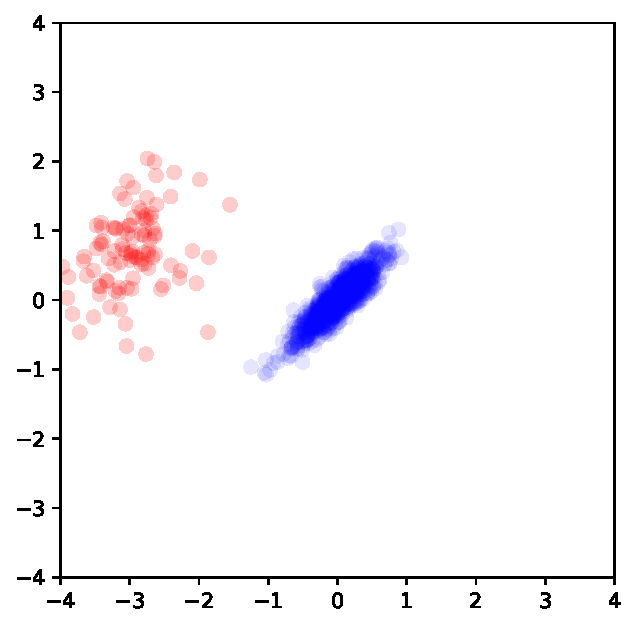
\includegraphics[width=\figw]{hw2/codes/gan/plots/alternating/0.pdf} &   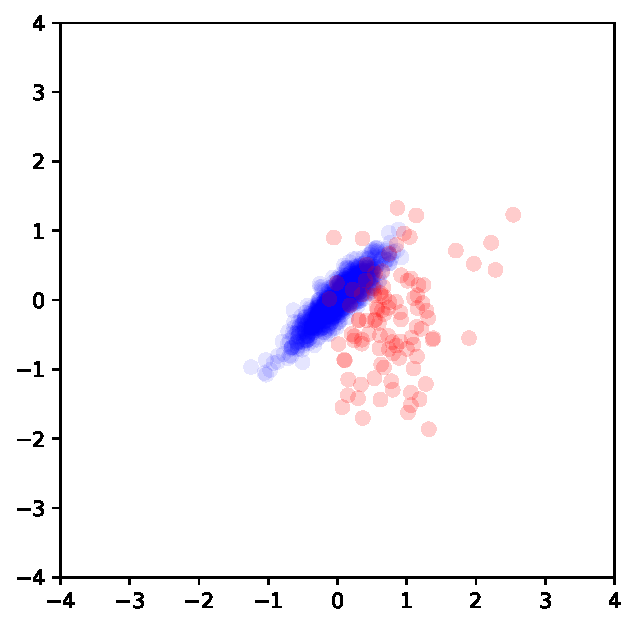
\includegraphics[width=\figw]{hw2/codes/gan/plots/alternating/1.pdf} \\
Start & 100th iteration \\[6pt]
 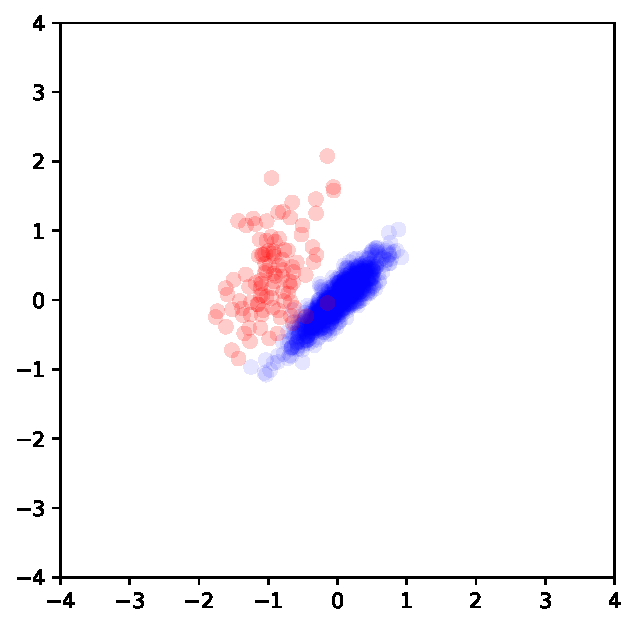
\includegraphics[width=\figw]{hw2/codes/gan/plots/alternating/2.pdf} &   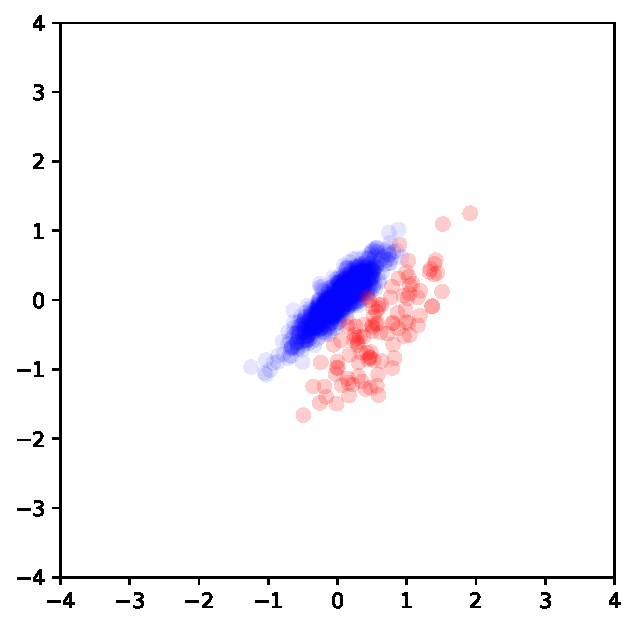
\includegraphics[width=\figw]{hw2/codes/gan/plots/alternating/3.pdf} \\
300th iteration & 400th iteration \\[6pt]
\end{tabular}
\caption{Simultaneous updates GAN training results}  \label{fig:simultaneous}
\end{figure}

The results of simultaneous updates can be checked statically in figure \ref{fig:simultaneous} and dynamically in a GIF on \href{https://media.giphy.com/media/Lr4Ssh49A7AXT9csiO/giphy.gif}{Giphy}. The results obtained with alternating updates, instead, can be observed statically in figure \ref{fig:alternating} and dinamically on \href{https://media.giphy.com/media/W5UZp7dkwiT6UTH6CW/giphy.gif}{Giphy}. In both cases we can see that the noise (the red points) gets almost the shape of the real distribution (the blue points), but keeps oscillating around its mean. We will discuss the reason of this in \ref{subsub:zero-difference}.

\begin{figure}
\centering
\begin{tabular}{cc}
  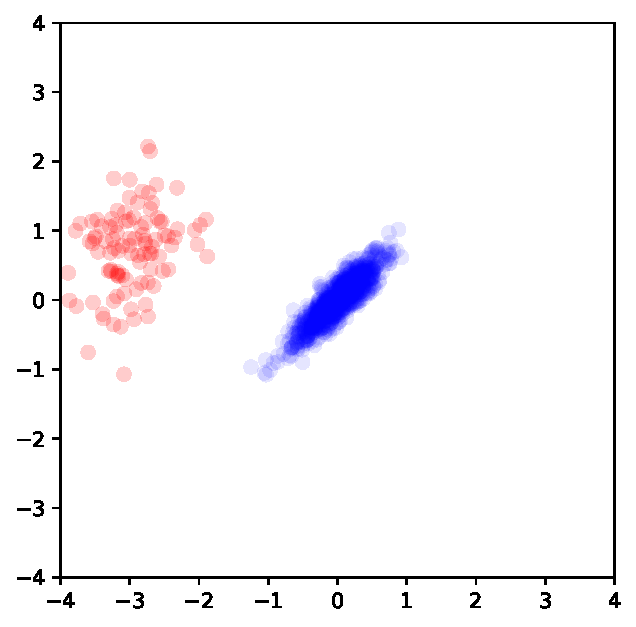
\includegraphics[width=\figw]{hw2/codes/gan/plots/simultaneous/0.pdf} &   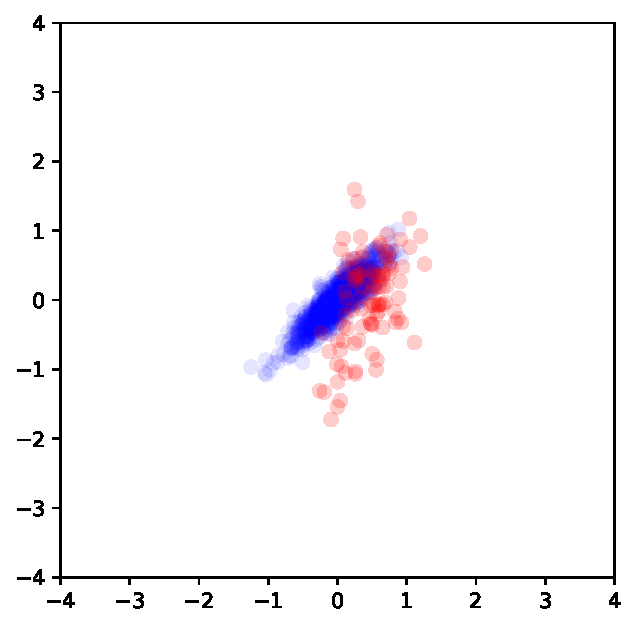
\includegraphics[width=\figw]{hw2/codes/gan/plots/simultaneous/1.pdf} \\
Start & 100th iteration \\[6pt]
 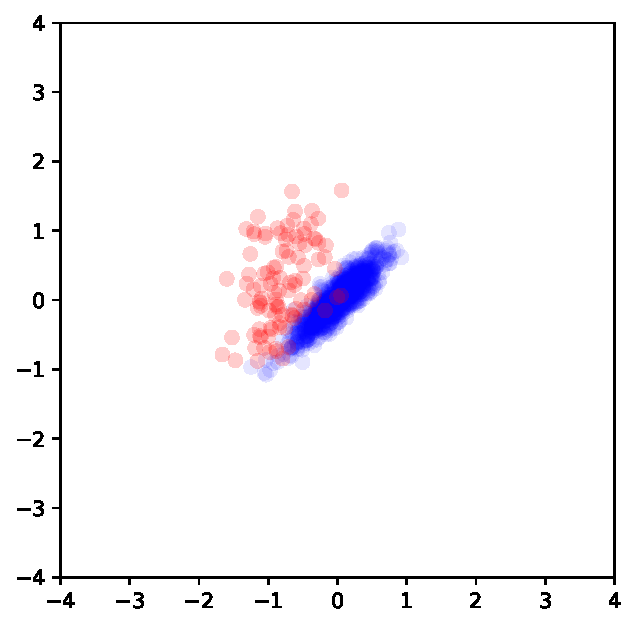
\includegraphics[width=\figw]{hw2/codes/gan/plots/simultaneous/2.pdf} &   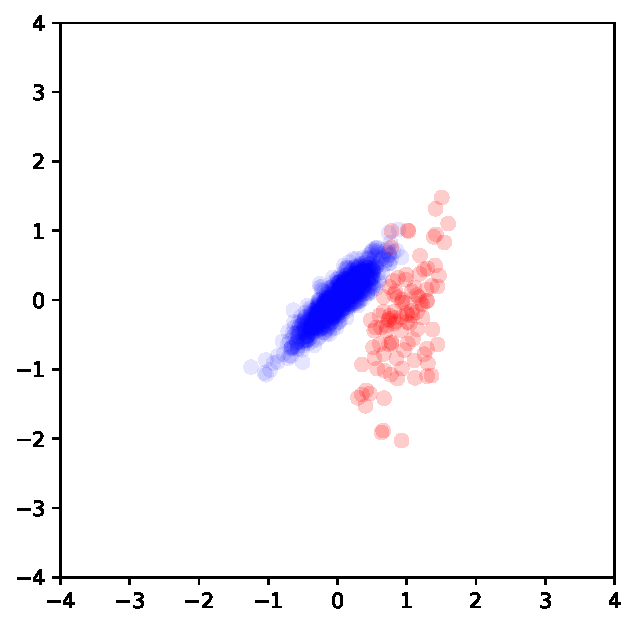
\includegraphics[width=\figw]{hw2/codes/gan/plots/simultaneous/3.pdf} \\
300th iteration & 400th iteration \\[6pt]
\end{tabular}
\caption{Alternating updates GAN training results} \label{fig:alternating}
\end{figure}

\subsubsection{max of expectation of difference of two distributions}
\begin{proof}
Given two distributions $\mu$ and $\nu$ and the class of functions $f \in \mathcal{F}$ we can prove that 
\begin{equation} \label{eq:exp-max-larger}
    \max_{f \in \mathcal{F}} \mathbb{E}_{X \sim \mu} [f(X)] -  \mathbb{E}_{Y \sim \nu} [f(Y)] \geq 0
\end{equation} \label{eq:expectation-ineq}
by first swapping the expectation operators with the function $f$, since both are linear:
\begin{gather}
    \max_{f \in \mathcal{F}} \mathbb{E}_{X \sim \mu} [f(X)] -  \mathbb{E}_{Y \sim \nu} [f(Y)] = \\
    \max_{f \in \mathcal{F}} f(\mathbb{E}_{X \sim \mu} [X]) -  f(\mathbb{E}_{Y \sim \nu} [Y]) = \label{eq:inner-exp}
\end{gather}
From now on, for the sake of simplicity we will write $\mathbb{E}_{X \sim \mu} [X]$ as $\Bar{X}$ and $\mathbb{E}_{Y \sim \nu} [Y]$ as $\bar{Y}$. We can also define the set of vectors $v \in \mathcal{V}_{1}$ which have norm $\lVert v \rVert \leq 1$ and then express eq. \eqref{eq:inner-exp} as
\begin{gather}
    \max_{v \in \mathcal{V}_1} v^{T}\Bar{X} -  v^{T}\Bar{Y} = \\
    \max_{v \in \mathcal{V}_1} v^{T}(\Bar{X} - \Bar{Y}) \label{eq:momentum-difference}
\end{gather}
Now we can consider different case, based on the different nature of the distributions. In the case where $\Bar{X} - \Bar{Y} = 0$, $\max_{v \in \mathcal{V}_1} v^{T}(\Bar{X} - \Bar{Y}) = 0$, which satisfies eq. \eqref{eq:exp-max-larger}. Otherwise, if $\Bar{X} - \Bar{Y} \lessgtr 0$, we can pick as $v \in \mathcal{V}_1$ the normal vector
\begin{equation} \label{eq:v}
    \hat{v} = \frac{\Bar{X} - \Bar{Y}}{\lVert \Bar{X} - \Bar{Y} \rVert}
\end{equation}
In such case,
\begin{gather}
    \hat{v}^{T}(\Bar{X} - \Bar{Y}) =
    \left ( \frac{\Bar{X} - \Bar{Y}}{\lVert \Bar{X} - \Bar{Y} \rVert} \right ) ^{T}(\Bar{X} - \Bar{Y}) = \\
    = \frac{\lVert \Bar{X} - \Bar{Y} \rVert ^{2}}{\lVert \Bar{X} - \Bar{Y} \rVert} = \lVert \Bar{X} - \Bar{Y} \rVert \geq 0
\end{gather}
Since eq. \eqref{eq:inner-exp} requires the max to be greater or equal than 0, we just need to find one $f$ that satisfies such condition, which is satisfied with $f = \hat{v}^{T}x$. However, since $\hat{v}$ is parallel to $\Bar{X} - \Bar{Y}$ and since is the largest vector that satisfies the 1-Lipschitz condition, is the vector that maximizes the product $v^{T}(\Bar{X} - \Bar{Y})$ which means

\begin{equation}
    \hat{v} \in \{v : \max_{v \in \mathcal{V}_1} v^{T}(\Bar{X} - \Bar{Y})\}
\end{equation}
\end{proof}

\subsubsection{0 max with equal first momentum} \label{subsub:zero-difference}
\begin{proof}
If we consider the left side of the inequality defined in \eqref{eq:expectation-ineq}, and we assume the first moment of $\mu$ and $\nu$ to coincide, then $\mathbb{E}_{X \sim \mu} [X] =  \mathbb{E}_{Y \sim \nu} [Y]$, since $X$ and $Y$ are two random variables drawn from $\mu$ and $\nu$. This leads to the case in eq. \eqref{eq:momentum-difference} where $\bar{X} - \bar{Y} = 0$ (recalling that $\mathbb{E}_{X \sim \mu} [X] = \bar{X}$ and $\mathbb{E}_{Y \sim \nu} [Y] = \bar{Y}$). Hence $\max_{v \in \mathcal{V}_1} v^{T}(\Bar{X} - \Bar{Y}) = 0$, which satisfies the required hypothesis.
\end{proof}

\paragraph{Update non-convergence study}
In the case of the simultaneous update, we update $f$ and $g$ together, which means that we simultaneously try to minimize Wasserstein distance over the generator $g$ and to compute the Wasserstein distance maximizing the difference between the expectations over the dual variable $f$. Instead, in the case of alternating updates, we first maximize the difference between the expectations over the dual variable $f$ to compute Wasserstein distance, and then we try to minimize Wasserstein distance over the generator $g$.

We can see from figure \ref{fig:alternating} that the real behavior of the generated data is oscillating around the mean, which means that $\mathbb{E}_{Z \sim \nu} [f(g(Z))]$ oscillates around $\mathbb{E}_{X \sim \mu} [f(X)]$, and then, since $f$ is linear, we can say that $\mathbb{E}_{Z \sim \nu} [g(Z)]$ oscillates around $\mathbb{E}_{X \sim \mu} [X]$. This is evident also in figure \ref{fig:objectives}, where we can see how the objective oscillates around 0 in both kinds of updates. Using alternating updates lead to a more oscillatory behavior, but the trend is the same. This is caused by the fact that, when the noise $Z$ is mapped to a distribution that has the same expectation as $X$ does, then $\max_{f \in \mathcal{F}} \mathbb{E}_{X \sim \mu} [f(X)] - \mathbb{E}_{Z \sim \nu} [f(g(Z)] = 0$, according to what we proved above. However, $g$ will still be updated to minimize the objective function (that can get negative values), leading to values smaller than 0, until the dual variable counteracts the observed behavior, causing the observed oscillatory behavior. A possible solution to this problem could be to take in consideration also higher order momenta for the distributions (such as variance).

\begin{figure}
\centering
\begin{tabular}{cc}
  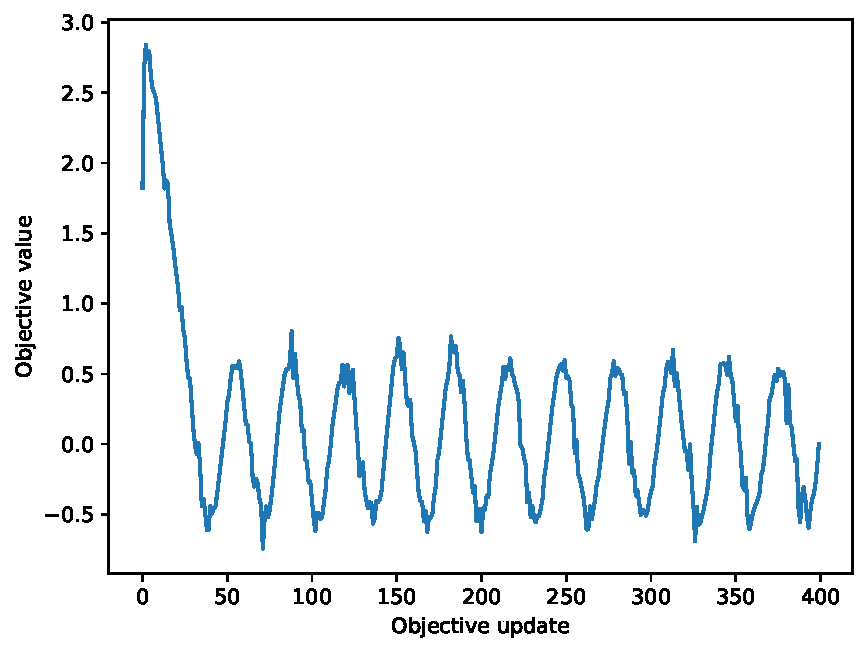
\includegraphics[width=\figw]{hw2/codes/gan/plots/simultaneous/simultaneous_objectives.pdf} &   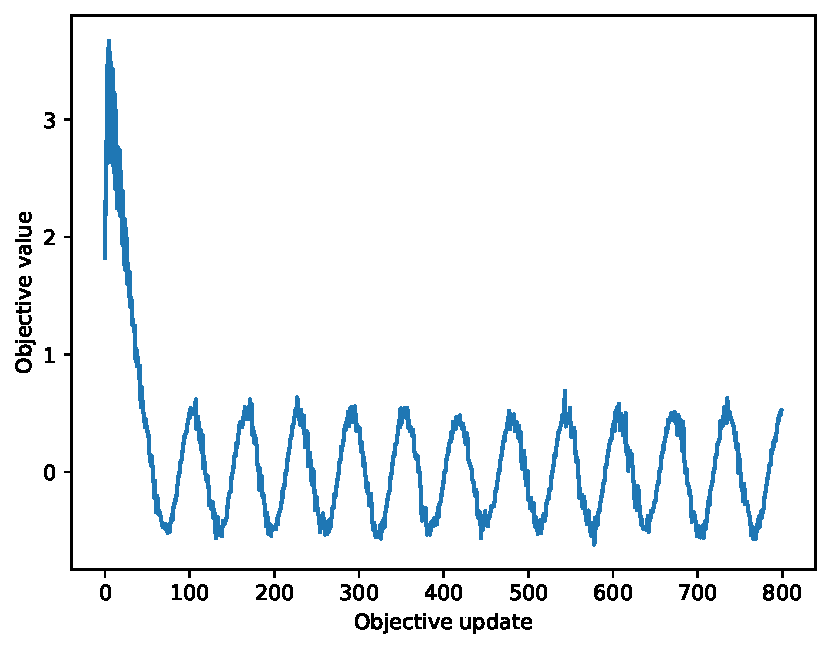
\includegraphics[width=\figw]{hw2/codes/gan/plots/alternating/alternating_objectives.pdf} \\
Simultaneous updates objective & Alternating updates objective \\[6pt]
\end{tabular}
\caption{GAN training objective behavior} \label{fig:objectives}
\end{figure}

\section{Optimizers of Neural Networks}

From the plots in figures \ref{fig:nn-1e-5}, \ref{fig:nn-1e-2}, \ref{fig:nn-0-5} and from the tables \ref{tab:1e-5}, \ref{tab:1e-2}, \ref{tab:0-5}, we can see that, in general, the best performing learning rate is $10^{-2}$. In fact, the only two methods that converge fast enough with l.r. $10^{-5}$ are ADAM and RMSProp. On the other side, the only two algorithms that do not suffer from the larger 0.5 learning rate are regular SGD and AdaGrad. Moreover, it is worth noting that with 0.5 l.r. the loss decreases quite fast for all the methods, but the accuracy does not increase for all of them. This phenomenon could be caused by overfitting on the loss function. In a classification task like the one our neural network is performing is more important to use the accuracy than the loss as a performance metric (even though accuracy could have strong limitations due to class proportions in the dataset in use).

In general, adaptive gradient methods perform slightly better and are more robust to different learning rates, even though we have some noteworthy differences among them. As a matter of fact, AdaGrad does not perform well enough with a too small learning rate, which can be caused by the stronger weight given to older gradients. Older gradients could lead to a more \textit{conservative} behavior that slows down AdaGrad's convergence. On the other side, this \textit{conservative} behavior improves AdaGrad's performance with the significantly larger 0.5 stepsize, for which we get acceptable enough performance.

\begin{table}
\centering
\begin{tabular}{l|l|l|l|l|l|l|l|l|}
\cline{2-9}
 & \multicolumn{2}{c|}{1st run} & \multicolumn{2}{c|}{2nd run} & \multicolumn{2}{c|}{3rd run} & \multicolumn{2}{c|}{Mean} \\ \hline
\multicolumn{1}{|l|}{Algorithm} & \multicolumn{1}{c|}{Training} & \multicolumn{1}{c|}{Test} & \multicolumn{1}{c|}{Training} & \multicolumn{1}{c|}{Test} & \multicolumn{1}{c|}{Training} & \multicolumn{1}{c|}{Test} & \multicolumn{1}{c|}{Training} & \multicolumn{1}{c|}{Test} \\ \hline
\multicolumn{1}{|l|}{SDG} & 0.1251 & 0.122 & 0.1177 & 0.115 & 0.1012 & 0.095 & \textbf{0.1147} & \textbf{0.1107} \\ \cline{1-1}
\multicolumn{1}{|l|}{SDGm} & 0.1915 & 0.2005 & 0.107 & 0.1101 & 0.2792 & 0.2887 & \textbf{0.1926} & \textbf{0.1998} \\ \cline{1-1}
\multicolumn{1}{|l|}{RMSProp} & 0.9134 & 0.9162 & 0.9131 & 0.918 & 0.9129 & 0.9167 & \textbf{0.9131} & \textbf{0.9170} \\ \cline{1-1}
\multicolumn{1}{|l|}{ADAM} & 0.9162 & 0.9183 & 0.917 & 0.9201 & 0.9171 & 0.9194 & \textbf{0.9168} & \textbf{0.9193} \\ \cline{1-1}
\multicolumn{1}{|l|}{AdaGrad} & 0.3218 & 0.3205 & 0.3969 & 0.4084 & 0.3904 & 0.3964 & \textbf{0.3697} & \textbf{0.3751} \\ \hline
\end{tabular}
\caption{Results obtained with learning rate $10^{-5}$}
\label{tab:1e-5}
\end{table}

\begin{figure}
\centering
\begin{tabular}{cc}
  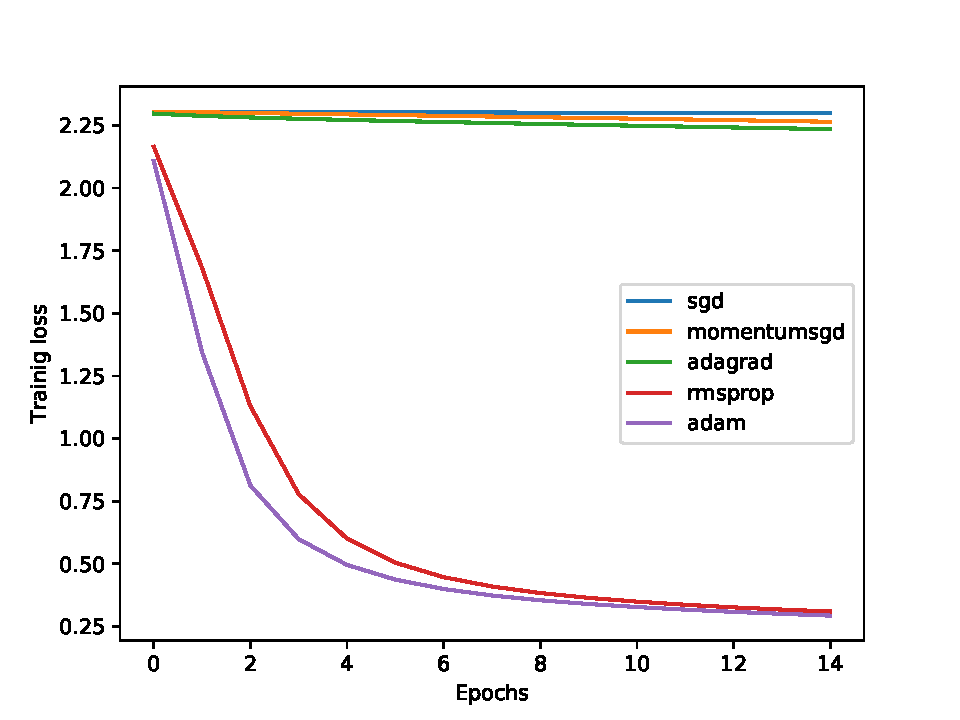
\includegraphics[width=\nnperfw]{hw2/codes/optimizer/pytorch/results/1e-5/loss.pdf} &   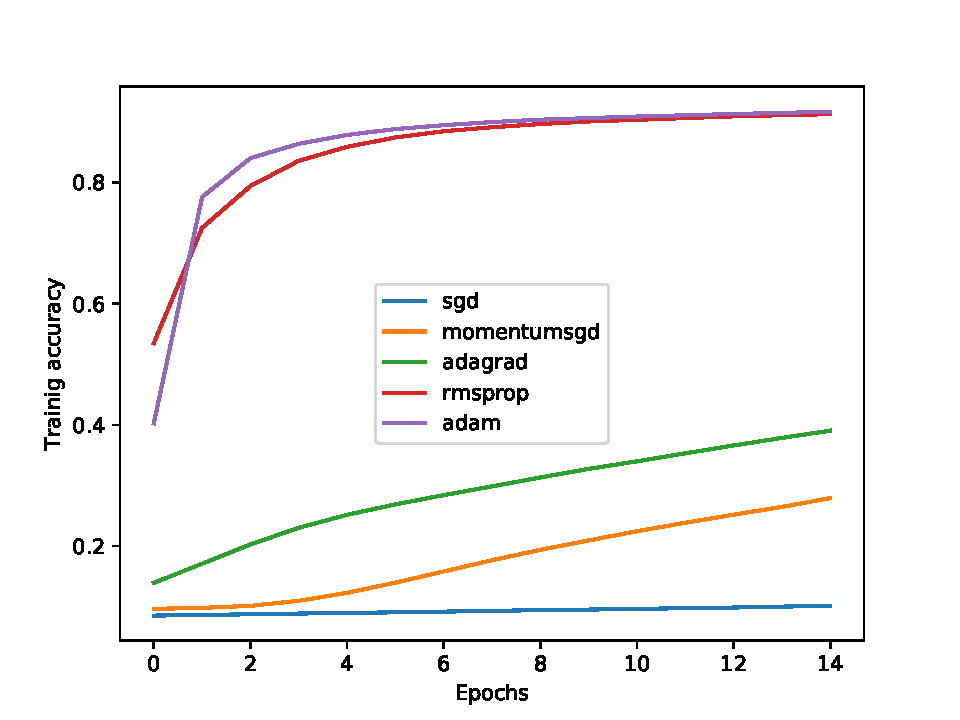
\includegraphics[width=\nnperfw]{hw2/codes/optimizer/pytorch/results/1e-5/accuracy.pdf} \\
Loss & Accuracy \\[6pt]
\end{tabular}
\caption{Performance with learning rate $10^{-5}$} \label{fig:nn-1e-5}
\end{figure}

\begin{table}
\centering
\begin{tabular}{l|l|l|l|l|l|l|l|l|}
\cline{2-9}
 & \multicolumn{2}{c|}{1st run} & \multicolumn{2}{c|}{2nd run} & \multicolumn{2}{c|}{3rd run} & \multicolumn{2}{c|}{Mean} \\ \hline
\multicolumn{1}{|l|}{Algorithm} & \multicolumn{1}{c|}{Training} & \multicolumn{1}{c|}{Test} & \multicolumn{1}{c|}{Training} & \multicolumn{1}{c|}{Test} & \multicolumn{1}{c|}{Training} & \multicolumn{1}{c|}{Test} & \multicolumn{1}{c|}{Training} & \multicolumn{1}{c|}{Test} \\ \hline
\multicolumn{1}{|l|}{SDG} & 0.9366 & 0.9372 & 0.9366 & 0.9396 & 0.936 & 0.9392 & \textbf{0.9364} & \textbf{0.9387} \\ \cline{1-1}
\multicolumn{1}{|l|}{SDGm} & 0.994 & 0.9792 & 0.9938 & 0.9791 & 0.9943 & 0.981 & \textbf{0.9940} & \textbf{0.9798} \\ \cline{1-1}
\multicolumn{1}{|l|}{RMSProp} & 0.9783 & 0.9676 & 0.9771 & 0.9617 & 0.9772 & 0.9617 & \textbf{0.9775} & \textbf{0.9637} \\ \cline{1-1}
\multicolumn{1}{|l|}{ADAM} & 0.985 & 0.9688 & 0.9858 & 0.9687 & 0.9872 & 0.9737 & \textbf{0.9860} & \textbf{0.9704} \\ \cline{1-1}
\multicolumn{1}{|l|}{AdaGrad} & 0.9978 & 0.9824 & 0.9975 & 0.9803 & 0.9977 & 0.9812 & \textbf{0.9977} & \textbf{0.9813} \\ \hline
\end{tabular}
\caption{Results obtained with learning rate $10^{-2}$}
\label{tab:1e-2}
\end{table}

\begin{figure}
\centering
\begin{tabular}{cc}
  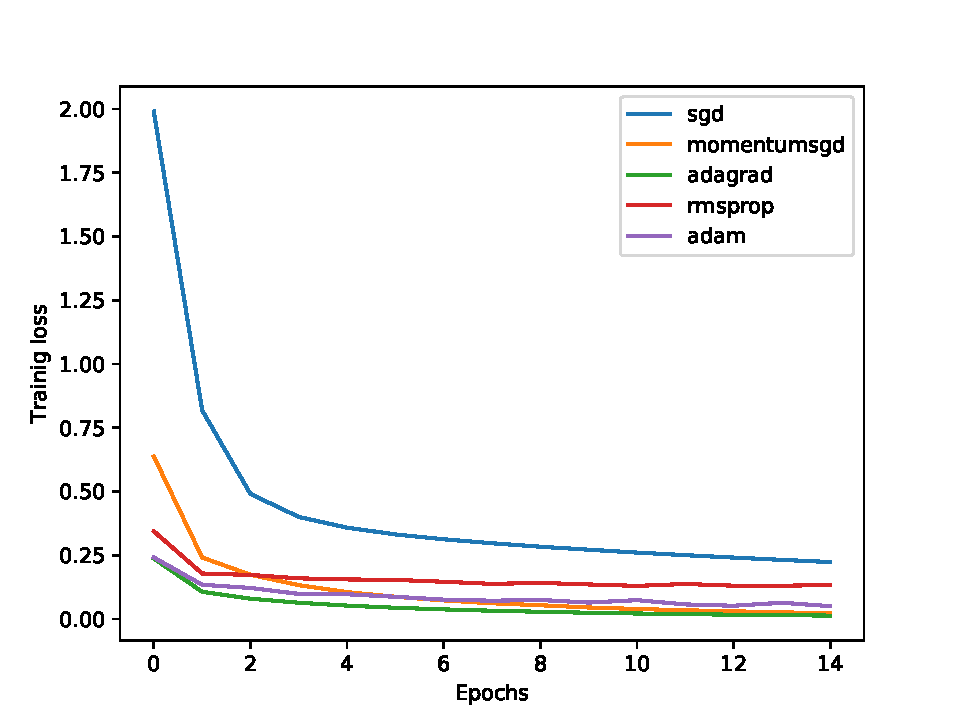
\includegraphics[width=\nnperfw]{hw2/codes/optimizer/pytorch/results/1e-2/loss.pdf} &   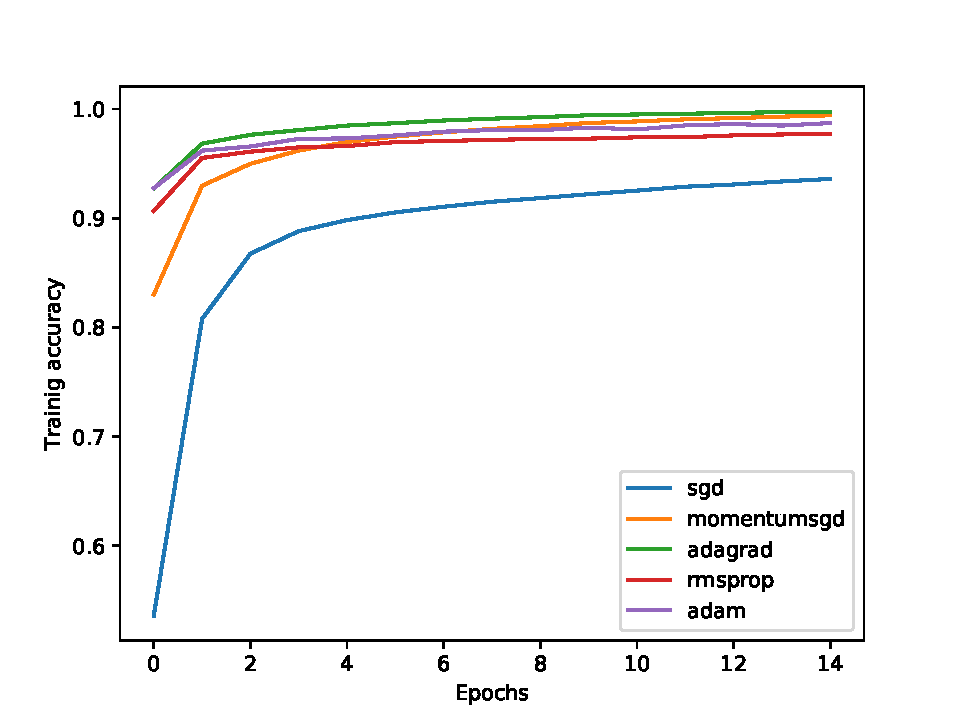
\includegraphics[width=\nnperfw]{hw2/codes/optimizer/pytorch/results/1e-2/accuracy.pdf} \\
Loss & Accuracy \\[6pt]
\end{tabular}
\caption{Performance with learning rate $10^{-2}$} \label{fig:nn-1e-2}
\end{figure}

\begin{table}
\centering
\begin{tabular}{l|l|l|l|l|l|l|l|l|}
\cline{2-9}
 & \multicolumn{2}{c|}{1st run} & \multicolumn{2}{c|}{2nd run} & \multicolumn{2}{c|}{3rd run} & \multicolumn{2}{c|}{Mean} \\ \hline
\multicolumn{1}{|l|}{Algorithm} & \multicolumn{1}{c|}{Training} & \multicolumn{1}{c|}{Test} & \multicolumn{1}{c|}{Training} & \multicolumn{1}{c|}{Test} & \multicolumn{1}{c|}{Training} & \multicolumn{1}{c|}{Test} & \multicolumn{1}{c|}{Training} & \multicolumn{1}{c|}{Test} \\ \hline
\multicolumn{1}{|l|}{SDG} & 0.9999 & 0.985 & 1 & 0.985 & 1 & 0.9839 & \textbf{1.0000} & \textbf{0.9846} \\ \cline{1-1}
\multicolumn{1}{|l|}{SDGm} & 0.2101 & 0.2144 & 0.1031 & 0.1135 & 0.1022 & 0.101 & \textbf{0.1385} & \textbf{0.1430} \\ \cline{1-1}
\multicolumn{1}{|l|}{RMSProp} & 0.1033 & 0.101 & 0.0995 & 0.1034 & 0.1027 & 0.1135 & \textbf{0.1018} & \textbf{0.1060} \\ \cline{1-1}
\multicolumn{1}{|l|}{ADAM} & 0.1031 & 0.1136 & 0.1036 & 0.0982 & 0.1031 & 0.1135 & \textbf{0.1033} & \textbf{0.1084} \\ \cline{1-1}
\multicolumn{1}{|l|}{AdaGrad} & 0.8418 & 0.8481 & 0.8972 & 0.8876 & 0.8944 & 0.8879 & \textbf{0.8778} & \textbf{0.8745} \\ \hline
\end{tabular}
\caption{Results obtained with learning rate $0.5$}
\label{tab:0-5}
\end{table}

\begin{figure}
\centering
\begin{tabular}{cc}
  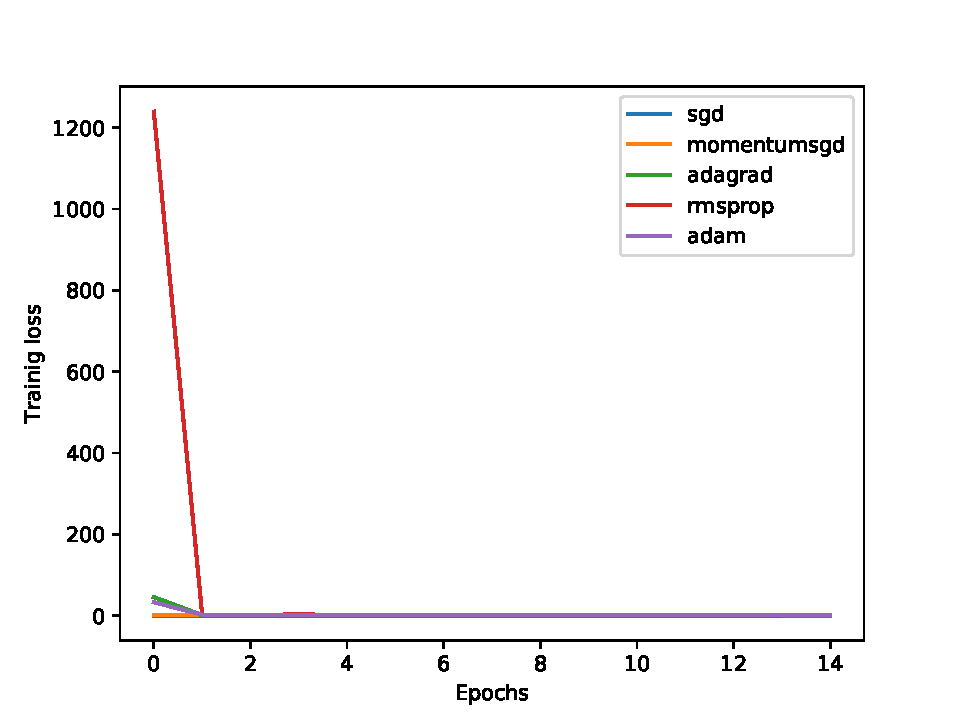
\includegraphics[width=\nnperfw]{hw2/codes/optimizer/pytorch/results/0_5/loss.pdf} &   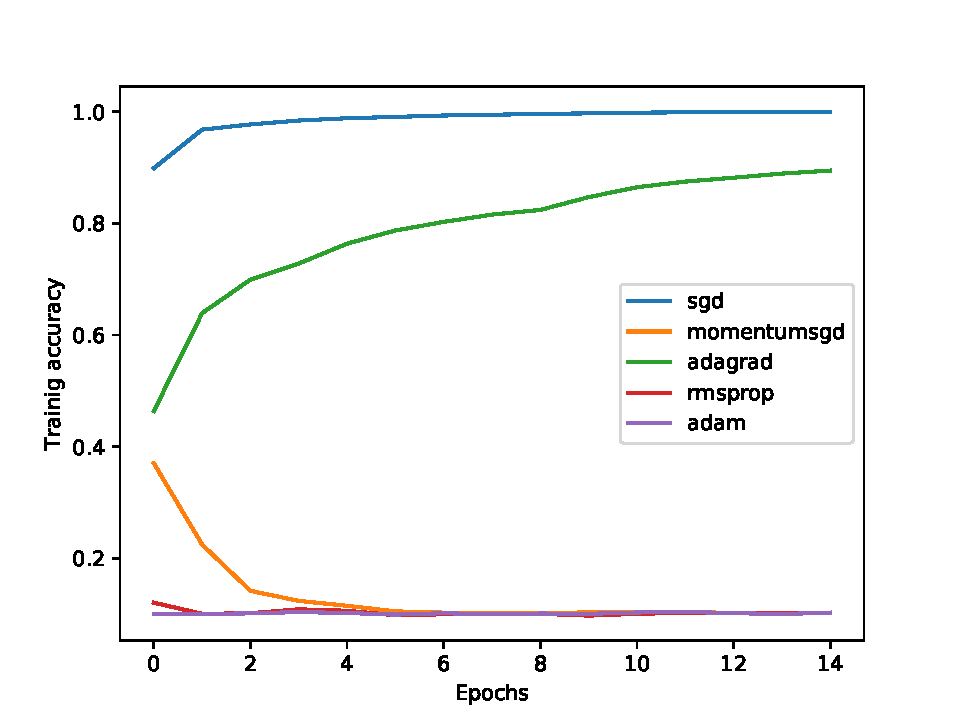
\includegraphics[width=\nnperfw]{hw2/codes/optimizer/pytorch/results/0_5/accuracy.pdf} \\
Loss & Accuracy \\[6pt]
\end{tabular}
\caption{Performance with learning rate $0.5$} \label{fig:nn-0-5}
\end{figure}

\end{document}